%% bpmlr.tex
%% V0.1
%% 2015/01/01
%% by Mack Sweeney

\documentclass[10pt]{proc}


% *** CITATION PACKAGES ***
%
\usepackage{cite}
% cite.sty was written by Donald Arseneau
% V1.6 and later of IEEEtran pre-defines the format of the cite.sty package
% \cite{} output to follow that of IEEE. Loading the cite package will
% result in citation numbers being automatically sorted and properly
% "compressed/ranged". e.g., [1], [9], [2], [7], [5], [6] without using
% cite.sty will become [1], [2], [5]--[7], [9] using cite.sty. cite.sty's
% \cite will automatically add leading space, if needed. Use cite.sty's
% noadjust option (cite.sty V3.8 and later) if you want to turn this off.
% cite.sty is already installed on most LaTeX systems. Be sure and use
% version 4.0 (2003-05-27) and later if using hyperref.sty. cite.sty does
% not currently provide for hyperlinked citations.
% The latest version can be obtained at:
% http://www.ctan.org/tex-archive/macros/latex/contrib/cite/
% The documentation is contained in the cite.sty file itself.


% *** OTHER BIBLIOGRAPHY PACKAGES ***
%
%\usepackage[numbers]{natbib}


% *** GRAPHICS RELATED PACKAGES ***
%
\usepackage[pdftex]{graphicx}
% declare the path(s) where your graphic files are
\graphicspath{{./graphics/}}
% and their extensions so you won't have to specify these with
% every instance of \includegraphics
\DeclareGraphicsExtensions{.pdf,.jpeg,.png}

\usepackage{scalerel}
\usepackage{mdframed}

% For graphical models:
\usepackage{tikz}
\usetikzlibrary{bayesnet}


% *** MATH PACKAGES ***
%
\usepackage[cmex10, fleqn]{amsmath}
\usepackage{bm}
\usepackage{bbm}
\usepackage{amssymb}
\usepackage{mathtools}
% A popular package from the American Mathematical Society that provides
% many useful and powerful commands for dealing with mathematics. If using
% it, be sure to load this package with the cmex10 option to ensure that
% only type 1 fonts will utilized at all point sizes. Without this option,
% it is possible that some math symbols, particularly those within
% footnotes, will be rendered in bitmap form which will result in a
% document that can not be IEEE Xplore compliant!
%
% Also, note that the amsmath package sets \interdisplaylinepenalty to 10000
% thus preventing page breaks from occurring within multiline equations. Use:
\interdisplaylinepenalty=2500
% after loading amsmath to restore such page breaks as IEEEtran.cls normally
% does. amsmath.sty is already installed on most LaTeX systems. The latest
% version and documentation can be obtained at:
% http://www.ctan.org/tex-archive/macros/latex/required/amslatex/math/


% *** SPECIALIZED LIST PACKAGES ***
%
\usepackage{algorithm}
\usepackage[noend]{algpseudocode}


% *** ALIGNMENT PACKAGES ***
%
\usepackage{array}
\usepackage{booktabs}
% Frank Mittelbach's and David Carlisle's array.sty patches and improves
% the standard LaTeX2e array and tabular environments to provide better
% appearance and additional user controls. As the default LaTeX2e table
% generation code is lacking to the point of almost being broken with
% respect to the quality of the end results, all users are strongly
% advised to use an enhanced (at the very least that provided by array.sty)
% set of table tools. array.sty is already installed on most systems. The
% latest version and documentation can be obtained at:
% http://www.ctan.org/tex-archive/macros/latex/required/tools/


% *** SUBFIGURE PACKAGES ***
%\usepackage[tight,footnotesize]{subfigure}
% subfigure.sty was written by Steven Douglas Cochran. This package makes it
% easy to put subfigures in your figures. e.g., "Figure 1a and 1b". For IEEE
% work, it is a good idea to load it with the tight package option to reduce
% the amount of white space around the subfigures. subfigure.sty is already
% installed on most LaTeX systems. The latest version and documentation can
% be obtained at:
% http://www.ctan.org/tex-archive/obsolete/macros/latex/contrib/subfigure/
% subfigure.sty has been superceeded by subfig.sty.

%\usepackage[caption=false]{caption}
%\usepackage[font=footnotesize]{subfig}
% subfig.sty, also written by Steven Douglas Cochran, is the modern
% replacement for subfigure.sty. However, subfig.sty requires and
% automatically loads Axel Sommerfeldt's caption.sty which will override
% IEEEtran.cls handling of captions and this will result in nonIEEE style
% figure/table captions. To prevent this problem, be sure and preload
% caption.sty with its "caption=false" package option. This is will preserve
% IEEEtran.cls handing of captions. Version 1.3 (2005/06/28) and later 
% (recommended due to many improvements over 1.2) of subfig.sty supports
% the caption=false option directly:
\usepackage[caption=false,font=footnotesize]{subfig}



% *** FLOAT PACKAGES ***
%
\usepackage{fixltx2e}
% fixltx2e, the successor to the earlier fix2col.sty, was written by
% Frank Mittelbach and David Carlisle. This package corrects a few problems
% in the LaTeX2e kernel, the most notable of which is that in current
% LaTeX2e releases, the ordering of single and double column floats is not
% guaranteed to be preserved. Thus, an unpatched LaTeX2e can allow a
% single column figure to be placed prior to an earlier double column
% figure. The latest version and documentation can be found at:
% http://www.ctan.org/tex-archive/macros/latex/base/

\usepackage{stfloats}
% stfloats.sty was written by Sigitas Tolusis. This package gives LaTeX2e
% the ability to do double column floats at the bottom of the page as well
% as the top. (e.g., "\begin{figure*}[!b]" is not normally possible in
% LaTeX2e). It also provides a command:
%\fnbelowfloat
% to enable the placement of footnotes below bottom floats (the standard
% LaTeX2e kernel puts them above bottom floats). This is an invasive package
% which rewrites many portions of the LaTeX2e float routines. It may not work
% with other packages that modify the LaTeX2e float routines. The latest
% version and documentation can be obtained at:
% http://www.ctan.org/tex-archive/macros/latex/contrib/sttools/
% Documentation is contained in the stfloats.sty comments as well as in the
% presfull.pdf file. Do not use the stfloats baselinefloat ability as IEEE
% does not allow \baselineskip to stretch. Authors submitting work to the
% IEEE should note that IEEE rarely uses double column equations and
% that authors should try to avoid such use. Do not be tempted to use the
% cuted.sty or midfloat.sty packages (also by Sigitas Tolusis) as IEEE does
% not format its papers in such ways.


% *** PDF, URL AND HYPERLINK PACKAGES ***
%
\usepackage{url}
% url.sty was written by Donald Arseneau. It provides better support for
% handling and breaking URLs. url.sty is already installed on most LaTeX
% systems. The latest version can be obtained at:
% http://www.ctan.org/tex-archive/macros/latex/contrib/misc/
% Read the url.sty source comments for usage information. Basically,
% \url{my_url_here}.


% BEGIN PAPER CONTENT
%
\title{Probabilistic Personalized Multi-Linear Regression}
\author{
    Mack Sweeney, Kathryn Laskey, Huzefa Rangwala\\
        George Mason University
}
\date{\today}


% New commands to be used in this report.
\newcommand*{\Scale}[2][4]{\scalebox{#1}{$#2$}}%
\newcommand*{\Resize}[2]{\resizebox{#1}{!}{$#2$}}%
\newcommand{\eqalign}[1]{{\footnotesize\begin{align}{#1}\end{align}}}
\newcommand{\norm}[1]{\left\lVert#1\right\rVert}
\newcommand{\pluseq}{\mathrel{+}=}
\newcommand{\mineq}{\mathrel{-}=}
\newcommand{\asteq}{\mathrel{*}=}
\newcommand{\elips}[1]{\ldots#1\allowbreak}
\newcommand{\bc}{,\allowbreak}

\newtheorem{lemma}{Lemma}
\newtheorem{proof}{Proof}

%\DeclareMathSizes{display size}{text size}{script size}{scriptscript size}.
\DeclareMathSizes{6}{6}{5}{4}


\begin{document}
\maketitle


\begin{abstract}

In \cite{elbadrawy_personalized_2015}, Elbadrawy et al. define a personalized
multi-linear regression model for predicting student performance in a
traditional university setting. This model is effectively a mixed-membership
linear regression. Student-specific and course-specific bias terms are learned.
Then several regression models are learned and combined in a linear combination
with student-specific membership weights. In this paper, we will replicate
that model and derive three distinct learning procedures. While the emphasis in
the original model was on non-negative parameter spaces, we allow negative
parameters to be learned and derive interpretable feature importance metrics for
this variation.

We begin with a Stochastic Gradient Descent (SGD) algorithm, then derive a
Coordinate Descent (CD) algorithm. Finally we interpet the model
probabilistically and derive a Markov Chain Monte Carlo (MCMC) sampling
procedure to learn the model parameters. Using our feature importance metrics,
we show how the parameters are learned differently using each method. This
exploration motivates a unique feature selection strategy applicable for any
regression model with additive components.

\end{abstract}


\section{Introduction}

\paragraph{Outline}
The remainder of this paper is organized as follows.
Section~\ref{previous work} gives account of previous work.
Our new and exciting results are described in Section~\ref{results}.
Finally, Section~\ref{conclusions} gives the conclusions.


\section{Personalized Multi-Linear Regression (PMLR)}

We begin by introducing the basic PMLR model
of~\cite{elbadrawy_personalized_2015} before generalizing the model to arbitrary
domains and feature spaces. Some of the notation is our own and some is from the
original model exposition. Let $S$ be the set of all students in our database
and $C$ be the set of all courses in our database. Further, let $G$ be the
matrix of all (student, course) dyads s.t. $G_{i,j}$ is the grade student $i \in
S$ obtained in course $j \in C$. Finally, let $\mathbb{I}$ be an indicator
matrix s.t.  $\mathbb{I}_{i,j} = 1$ if $G_{i,j}$ is a dyad in our database
(student $i$ has taken course $j$) and $\mathbb{I}_{i,j} = 0$ otherwise. Our
goal is to predict the grade a previously seen student will achieve in a
previously seen course. The original PMLR model is not equipped to handle
cold-start predictions (predicting grades for unseen students or for known
students on unseen courses). In order to facilitate conciseness of notation, we
define $n = |S|$ as the number of students, $m = |C|$ as the number of courses,
and $nz = \sum_{i=1}^N \sum_{i=j}^M \mathbb{I}_{i,j}$ as the number of non-zero
dyads $(i,j)$. In addition to the grades, we also observe dyad features
$\bm{D}^{n \times m \times p}$, such that entry $\bm{D}_{i,j}^{p \times 1}$ is
the feature vector observed for user $i$ on course $j$.

The PMLR model assumes the presence of $k$ general response profiles which
describe the observed users. Since each user might be described to a greater or
lesser extent by each general profile, user-specific membership vectors are
learned that operate as weights in a linear combination of the regression
outputs. When non-negativity constraints are introduced, learning these
membership weights can be thought of as clustering the users. The model further
assumes user- and item-specific biases. These biases are modeled as 1-way
interactions with the response variable. More concretely, the PMLR model is
comprised of four parameters:
%
\begin{itemize}
    \item  $\bm{s}^{n x 1}$ is the vector of student bias terms
    \item  $\bm{c}^{m x 1}$ is the vector of course bias terms
    \item  $P^{n x k}$ is the matrix of student membership vectors
    \item  $W^{k x p}$ is the matrix of linear regression coefficient vectors
\end{itemize}
%
Predictions are made using:
%
\begin{equation}
    \hat{g}(i,j) = \bm{s}_i + \bm{c}_j + P_i^T W \bm{D}_{i,j}.
\end{equation}
%
We say that the matrix $\hat{G}$ is the matrix of predicted grades, such that
$\hat{G}_{i,j} = \hat{g}(i, j)$.
%
The loss function is defined as the root mean squared error (RMSE):
%
\begin{align}
    l(i,j) &= (G_{i,j} - \hat{G}_{i,j})^2 \mathbb{I}_{i,j},  \\
    \mathcal{L} &= \norm{G - \hat{G}}^2
\end{align}
%
and the squared Frobenius norm is used for regularization on the membership
weights $P$ and the regression coefficient matrix $W$:
%
\begin{align}
    r(i,j) &= \lambda (\norm{P_i}_F^2 + \norm{W}_F^2) \mathbb{I}_{i,j}  \\
    \mathcal{R} &= \lambda (\norm{P}_F^2 + \norm{W}_F^2).
\end{align}
%
For convenience of notation, we group the bias terms into the set $B = \{\bm{s},
\bm{c}\}$. The overall objective function minimizes the sum of loss and the
regularization term over parameters:
%
\begin{align}
    \underset{B, P, W}{\text{minimize}}
        \sum_{i=1}^n \sum_{j=1}^m l(i,j) + r(i,j)
\end{align}

In the original model, non-negativity constraints are placed on all model
parameters in order to enhance interpretability:
%
\begin{align}
  \begin{split}
    W_{l,f}  &\ge 0, 1 \le l \le k, 1 \le f \le p  \\
    P_{i,l}  &\ge 0, 1 \le l \le k, \forall i      \\
    \bm{s}_i &\ge 0, \forall i                     \\
    \bm{c}_j &\ge 0, \forall j
  \end{split}
\end{align}


\section{Individualized Profile Regression}

In this section we generalize the PMLR model to arbitrary domains and move from
a matrix factorization setting to a more general tensor factorization setting.
We call the resulting model Individualized Profile Regression (IPR).

First we observe that the PMLR model is directed at solving the matrix
completion problem. Given a partially observed matrix $R$, the task is to fill
in the missing entries. This observation places the PMLR model in the
recommender systems domain. We observe users producing responses for items
through some process. The response user $i$ produces for item $j$ is placed in
entry $R_{i,j}$. In this case, we also observe additional side information for
each user-item combination, stored in $\bm{D}$. Given side information, the
recommender systems problem can also be cast more generally as a dyadic response
prediction problem. To do so, we would simply assign each of our observed dyads
a unique identifier and fold all user and item ids into the feature vectors.
However, we move forward with the recommender systems notation, since we find it
is more natural to separate the bias terms from the other features.

We now motivate the desire to further generalize this model. The notion of
personalization here is modeled through the user-specific membership weights.
Imagine that we would instead like to capture general profiles for another
entity. For instance, we might believe latent item profiles have more predictive
power for the responses in a particular domain. In this case, we can simply swap
the user and item ids in the model equation. Then we capture item-specific
membership weights for the profiles. The same procedure works for any arbitrary
entity we might observe.

Next consider the effect of the bias terms in the predictive function. If our
goal is to learn general response profiles, we would like to remove variance
that is caused by less general patterns in the data. The user-specific bias
terms serve to remove user-specific variance in responses. What about the
item-specific bias terms? One could argue that general user response profiles
could incorporate general response patterns to particular items. However, we
expect item side information to be more useful for exploiting item-specific
response patterns. So we use the item features in the response profile and
capture variance which is not explained by the observed features in a bias term.
This approach facilitates the goal of feature interpretability in the response
profiles. It also allows us to see how much item-specific variance is not
captured by the features we have observed. This insight can help us determine to
some extent how much user responses to items are explainable through the
observed features and how much has yet to be explained.

If we extend this line of thinking to additional entities, we gain an intuitive
procedure for extending the model. For each additional entity observed, we
should place any side information related to the entity inside the profile
feature vectors and introduce additional entity-specifc bias terms. Through this
procedure, we can move from predicting for dyads to predicting for triads and
beyond. In the recommender systems setting, we move from matrix completion to
more general tensor completion.

We call this generalized model Individualized Profile Regression.  We define $e$
as the number of entities we are learning bias terms for and $b_1, ..., b_e$ as
the number of distinct values for each entity. We index into these dimensions
using indices $i_1, ..., i_e$. By convention, we profile for the first entity
and use $i$ as a shorthand for $i_1$.  We denote the total number of bias terms
as $b^*$. In order to simplify tensor indexing notation, we use a special index
$t = i_1, ..., i_e$ to index into tensors. We also define a custom dimension $d
= b_1 \times ... \times b_e$ to denote the dimensionality of our tensors. We
store our one-hot encoded entity features in tensor $\bm{B}^d$, the rest of our
features in tensor $\bm{X}^d$, and our responses in tensor $\bm{Y}^d$. For
entity combination $t$, $\bm{B}_t^{b^* \times 1}$ contains all bias terms,
$\bm{X}_t^{p \times 1}$ is the feature vector, and $\bm{Y}_t$ is the scalar
response.

Let us now formalize the notions we have been discussing. We define four
parameters for the IPR model. We differ from the PMLR model by introducing a
global intercept term. All bias terms are folded into a single vector and $P$
and $W$ remain the same.
%
\begin{itemize}
    \item  $w_0$ is the global intercept term,
    \item  $\bm{w}^{b^* \times 1}$ is the vector of bias terms,
    \item  $P^{b_1 \times k}$ is the matrix of entity membership vectors,
    \item  $W^{k \times p}$ is the matrix of linear regression coefficient vectors.
\end{itemize}
%
Hence our parameter space consists of $\mathrel{\theta \in \Theta = \{}w_0\bc
\bm{w}_1\bc \elips{,} \bm{w}_{b^*}\bc P_{1,1}\bc \elips{,} P_{1,k}\bc \elips{,}
P_{b_1,k}\bc W_{1,1}\bc \elips{,} W_{k,1}\bc \elips{,} W_{k,p}\}$.  For a particular
observation $t$, we predict the response using:
%
\begin{align}
    \hat{y}(t | \Theta)
        &= w_0 + \sum_{f=1}^{b^*} \bm{w}_f \bm{B}_{t,f} +
           \sum_{l=1}^m P_{i,l} \sum_{f=1}^p W_{l,f} \bm{X}_{t,f}  \\
        &= w_0 + \bm{w}^T \bm{B}_t + P_i^T W \bm{X}_t
\end{align}
%
We are interested in minimizing the loss, defined as the RMSE over all
observations. For this purpose, we define an indicator tensor $\mathbbm{I}^d$,
where entry $\mathbbm{I}_t = 1$ if we have observed entity combination $t$ and
$\mathbbm{I}_t = 0$ otherwise. Finally, we define the set of all entry indices
which are observed (for which $\mathbbm{I}_t = 1$) as $A$. With the use of the
indicator, we define the RMSE for IPR as:
%
\begin{align}
    l(t) &= (\bm{Y}_t - \hat{y}(t))^2  \\
    \mathcal{L} &= \sum_{t \in A} l(t).
\end{align}
%
We use the same regularization scheme as in PMLR:
%
\begin{align}
    r(t) &= \lambda (\norm{P_i}_F^2 + \norm{W}_F^2)  \\
    \mathcal{R} &= \sum_{t \in A} r(t).
\end{align}
%
And our objective function is the usual loss plus regularization.
%
\begin{align}
    f(t) &= l(t) + r(t)  \\
    \mathcal{F} &= \sum_{t \in A}  \label{eq:ipr-opt}
        (\bm{Y}_t - \hat{y}(t))^2 + \lambda (\norm{P_i}_F^2 + \norm{W}_F^2)
\end{align}
%
We solve this problem and learn our model by finding the parameter values
$\Theta$ that minimize our objective function:
%
\begin{align}
    &\underset{\Theta}{\text{argmin }} \mathcal{F}  \label{eq:obj}
\end{align}


\section{Learning Methods}

We derive three efficient procedures for learning the parameters
$\Theta$ of the IPR model. The first is a Stochastic Gradient Descent (SGD)
procedure, the second is deterministic Coordinate Descent (CD), also known as
ALS, and the third is a Markov Chain Monte Carlo (MCMC) algorithm. For MCMC, we
interpret the model probabilistically and derive an efficient Gibbs sampler for
inference. All three methods optimize via the objective function (\ref{eq:obj})
and will make use of some basic theoretical foundations which we lay
in~\ref{theoretical-foundations}.


\subsection{Theoretical Foundations} \label{theoretical-foundations}

In this section, we draw upon the work of Rendle et al. in
\cite{rendle_fast_2011} to prove several results that will be useful for
derivation of efficient learning procedures for the IPR model.

\begin{lemma}
    The IPR model equation $\mathcal{F}$ is linear with respect to every
    individual model parameter. Therefore we can represent it as a sum of
    multiplicative terms $\beta$ and additive terms $\alpha$, as follows:
%%
    \begin{equation}  \label{eq:yhat-decomp}
        \hat{y}(t | \theta) = \theta\beta_\theta(t) + \alpha_\theta(t).
    \end{equation}
\end{lemma}

\begin{proof}
    To prove this, we simply state $\beta$ and $\alpha$ explicitly for each
    $\theta \in \Theta$, decomposing (\ref{eq:ipr-opt}).
%%
    {\footnotesize
    \begin{flalign}
        \hat{y}(t | w_0) &= \begin{aligned}[t]  \label{eq:decomp-w0}
            w_0 \underbrace{(1)}_{\beta_{(w_0)}(t)} +
            \underbrace{
                \bm{w}^T \bm{B}_t + P_i^T W \bm{X}_t
            }_{\alpha_{(w_0)}(t)}
        \end{aligned} \\
%%
        \hat{y}(t | \bm{w}_f) &= \begin{aligned}[t]  \label{eq:decomp-w_f}
            & \bm{w}_f \overbrace{
                \bm{B}_{t,f}
            }^{\beta_{(\bm{w}_f)}(t)} + \\
            & \underbrace{
                w_0 + \sum_{f'=1, f' \neq f}^p \bm{w}_f' \bm{B}_{t,f'} +
                P_i^T W \bm{X}_t
            }_{\alpha_{(\bm{w}_f)}(t)}
        \end{aligned} \\
%%
        \hat{y}(t | P_{i,l}) &= \begin{aligned}[t]  \label{eq:decomp-P_il}
            & P_{i,l} \overbrace{
                W_l^T \bm{X}_t
            }^{\beta_{(P_{i,l})}(t)} + \\
          & \underbrace{
                w_0 + \bm{w}^T \bm{B}_t +
                \sum_{l'=1, l' \neq l}^k P_{i,l'} W_{l'}^T \bm{X}_t
            }_{\alpha_{(P_{i,l})}(t)}
        \end{aligned} \\
%%
        \hat{y}(t | W_{l,f}) &= \begin{aligned}[t]  \label{eq:decomp-W_lf}
            & W_{l,f} \overbrace{
                P_{i,l} \bm{X}_{t,f}
            }^{\beta_{(W_{l,f})}(t)} + \\
          & \underbrace{
                w_0 + \bm{w}^T \bm{B}_t +
                \sum_{l'=1}^k P_{i,l'}
                    \sum_{\mathrlap{\hspace{-5mm}
                        f'=1, (f' \neq f) \cup (l' \neq l)}}^p
                            W_{l',f'} \bm{X}_{t,f'}
            }_{\alpha_{(W_{l,f})}(t)}
        \end{aligned}
    \end{flalign}%
    }%
\end{proof}


\begin{lemma}
    The IPR model equation $f(t)$ is also linear with respect to the parameter
    vectors/matrices $\mathrel{\theta \in \Theta_t = \{} \bm{w}, P_i, W\}$.
    Therefore we can represent it as the same sum of multiplicative terms
    $\beta$ and additive terms $\alpha$ as in (\ref{eq:yhat-decomp}).
\end{lemma}

\begin{proof}
    Again the proof comes from simply stating $\beta$ and $\alpha$ for each
    $\theta$.
%%
    {\footnotesize
    \begin{flalign}
        \hat{y}(t | \bm{w}) &= \begin{aligned}[t]  \label{eq:decomp-w}
            \bm{w}^T \underbrace{(\bm{B}_t)}_{\beta_{(w_0)}(t)} +
            \underbrace{
                w_0 + P_i^T W \bm{X}_t
            }_{\alpha_{(\bm{w})}(t)}
        \end{aligned} \\
%%
        \hat{y}(t | P_i) &= \begin{aligned}[t]  \label{eq:decomp-P_i}
            & P_i^T \underbrace{
                W \bm{X}_t
            }_{\beta_{(P_i)}(t)} +
            \underbrace{
                w_0 + \bm{w}^T \bm{B}_t
            }_{\alpha_{(P_i)}(t)}
        \end{aligned} \\
%%
        \hat{y}(t | W) &= \begin{aligned}[t]  \label{eq:decomp-W}
            W \mathrel{.*} \underbrace{
                P_i \bm{X}_t^T
            }_{\beta_{(W)}(t)} +
            \underbrace{
                w_0 + \bm{w}^T \bm{B}_t
            }_{\alpha_{(W)}(t)}
        \end{aligned},
    \end{flalign}%
    }%
%
    where the operator $\mathrel{.*}$ is borrowed from Matlab and denotes
    elementwise matrix multiplication.
\end{proof}

Finally, we note that computation of $\alpha_\theta(t)$ takes time
$O(|\Theta|)$, where $|\Theta| = b^* b_1 k + pk)$ for $\theta \in \Theta$, while
computation of $\beta_\theta(t)$ takes constant time. So computation of
$\hat{y}(t)$ takes time $O(|\Theta|)$. The results in this section will be
useful for the learning procedures described below.


\subsection{SGD Algorithm}

We now introduce an SGD procedure for learning the parameters of the model. SGD
updates each parameter for every training example. Given a learning rate
$\alpha$ and a regularization term $\lambda_\theta$ for each parameter $\theta$,
we update each parameter in the direction of its partial derivative with respect
to $f(t)$:
%
\begin{align}
    \theta^* =
        \theta - 2\alpha \left(
            e(t | \Theta) \beta_\theta(t) + \theta\lambda_\theta
        \right),
\end{align}
%
where $e(t | \Theta)$ is the error $\bm{Y}_t - \hat{y}(t)$.

We update the feature vectors all at once, making use of (\ref{eq:decomp-w0}),
(\ref{eq:decomp-w}), (\ref{eq:decomp-P_i}), and (\ref{eq:decomp-W}). We perform
each of these parameter updates for all observed instances $A$. The procedure
requires a learning rate $\alpha$, a regularization constant $\lambda$, and an
initial standard deviation $\sigma$, which is used for parameter initialization.
We must also specify the number of iterations $\phi$ and the number of models
$k$. A stopping threshold $\epsilon$ can also be specified for early stopping.
At the end of each loop, we shuffle $A$ so we loop through the observations in a
random order on subsequent iterations. We set $\lambda_{(w_0)} =
\lambda_{(\bm{W})} = 0$ and set $\lambda_{(P_i)} = \lambda_{(W)} = \lambda$.

\begin{algorithm}  \label{alg:ipr-sgd}
    \caption{IPR-SGD($\bm{B}, \bm{X}, \bm{Y}, \alpha, \lambda, \sigma, \phi, k[, \epsilon]$)}
    \begin{algorithmic}[1]
        \State $\bm{w}, P, W \sim \mathcal{N}(0, \sigma)$
        \State $\alpha = 2 \alpha$
        \For{iteration in $\{1, \elips{,} \phi\}$}
            \For{$t \in A$}
                \State $e(t | \Theta) = \bm{Y}_t - \hat{y}(t)$
                \State $w_0 \mineq \alpha e(t | \Theta)$
                \State $\bm{w} \mineq \alpha e(t | \Theta)\bm{B}_t$
                \State $P_i \mineq \alpha (e(t | \Theta) W \bm{X}_t + \lambda P_i)$
                \State $W \mineq \alpha (e(t | \Theta) P_i \bm{X}_t^T + \lambda W)$
            \EndFor
            \State Shuffle $A$
            \If{$\epsilon$ given}
                \State compute RMSE; early stopping check
            \EndIf
        \EndFor
    \end{algorithmic}
\end{algorithm}

Computation of $e(t | \Theta)$ takes time $O(|\Theta|)$, and each update takes
constant time. So a single iteration takes time $O(|\Theta|)$, and one pass
through the training data takes time $O(|A||\Theta|)$. The total complexity of
the algorithm is $O(\phi|A||\Theta|)$, which is linear in the number of
iterations, training examples, and parameters.

\subsection{CD Algorithm}

CD learning operates by learning each parameter $\theta$ in isolation with all others
$\Theta / \theta$ fixed. For each, we fix all the others and solve for the value
that minimizes the objective function in closed form. As we move through the
parameters, we keep track of the residual error and train on that. In this way,
the earlier parameters have the opportunity to observe more of the variance that
accounts for the error. For each parameter $\theta \in \Theta$, we derive closed
form solutions. Rather than updating $P$ and $W$ one row at a time, as we do
with SGD, we update them one entry at a time.

\begin{lemma}
    (Optimal value for $\theta$) The regularized least-squares solution of a
    single parameter $\theta$ given all other parameters $\Theta / {\theta}$ for
    a linear model $\hat{y}(t| \Theta / {\theta})$ is:
%%
    \begin{equation}  \label{eq:theta-update}
        \theta =
            \frac{-\sum_{t \in A} (\bm{Y}_t - \alpha_\theta(t)) \beta_\theta(t)}
                 {\lambda_\theta - \sum_{t \in A} \beta_\theta^2(t)}
    \end{equation}
\end{lemma}

\begin{proof}
    To find the solution analytically, the first derivative of (\ref{eq:obj})
    w.r.t $\theta$ must be found:
%%
    \begin{equation} \label{eq:ipr-obj-derivative}
        \frac{ \partial \mathcal{F}}{ \partial\theta } =
            \sum_{t \in A} 2(\bm{Y}_t - \hat{y}(t)) \beta_\theta(t) +
            2\theta\lambda_\theta
    \end{equation}
%%
    The minimum is where this derivative is equal to 0:
%%
    {\footnotesize
    \begin{align*}
        & \hphantom{==} \begin{aligned}[t]
            0 &=
            \sum_{t \in A} 2(\bm{Y}_t - \hat{y}(t)) \beta_\theta(t) +
            2\theta\lambda_\theta
        \end{aligned} \\
        & \Leftrightarrow \begin{aligned}[t]
            0 &=
            \sum_{t \in A} (\bm{Y}_t - \theta\beta_\theta(t) - \alpha_\theta(t))
                \beta_\theta(t) +
                \theta\lambda_\theta
        \end{aligned} \\
        & \Leftrightarrow \begin{aligned}[t]
            0 &=
            \sum_{t \in A} (\bm{Y}_t - \alpha_\theta(t)) \beta_\theta(t) +
            \theta \left(\lambda_\theta - \sum_{t \in A} \beta_\theta^2(t)\right)
        \end{aligned} \\
        & \Leftrightarrow \begin{aligned}[t]
            \theta &=
                \frac{-\sum_{t \in A} (\bm{Y}_t - \alpha_\theta(t)) \beta_\theta(t)}
                     {\lambda_\theta - \sum_{t \in A} \beta_\theta^2(t)}
        \end{aligned}
    \end{align*}%
    }%
\end{proof}

Working from the results in Section \ref{theoretical-foundations}, we see that
(\ref{eq:theta-update}) takes time $O(|A||\Theta|)$. A single iteration in
which we update all parameters would take time $O(|\Theta|^2|A|)$, which is
quadratic in the number of parameters. We can improve this if we precompute the
error terms for each observation $e(t | \Theta)$.
%
\begin{align}
    & \hphantom{==} \begin{aligned}[t]
        e(t | \Theta)
            &= \bm{Y}_t - \hat{y}(t)  \\
            &= \bm{Y}_t - \theta\beta_\theta(t) - \alpha_\theta(t)
    \end{aligned} \\
    & \Leftrightarrow \begin{aligned}[t]
        e(t | \Theta) - \theta\beta_\theta(t)
            &= \bm{Y}_t - \alpha_\theta(t)
    \end{aligned}
\end{align}
%
Having done this in time $O(|\Theta||A|)$, we can now compute the updates for
each parameter in time $O(|A|)$ and complete a single iteration of updates in
time $O(|\Theta||A|)$. We simply reformulate (\ref{eq:theta-update}) as:
%
\begin{align} \label{eq:theta-star-update}
    \theta^* =
    \frac{-\sum_{t \in A} (e(t | \Theta) - \theta\beta_\theta) \beta_\theta(t)}
         {\lambda_\theta - \sum_{t \in A} \beta_\theta^2(t)},
\end{align}
%
where $\theta^*$ is the new value for $\theta$. After updating a parameter, we
simply update our error cache and parameter value with:
%
\begin{align}
    e(t | \Theta) &\pluseq (\theta - \theta^*) \beta_\theta(t) \\
    \theta &= \theta^*.
\end{align}
%
The calculation of (\ref{eq:theta-star-update}) takes time $O(|A|)$ and the
subsequent error update takes time $O(1)$, so we can now update all features in
$O(|\Theta||A|)$, which is linear in the number of parameters and training
instances. The CD algorithm is listed in Algorithm \ref{alg:ipr-cd}. Notice that
we no longer require a learning rate $\alpha$. The other parameters remain the
same as in SGD. To update the parameters, we use equations
(\ref{eq:decomp-w0}) to (\ref{eq:decomp-W_lf}).

\begin{algorithm}[tb]
    \caption{IPR-CD($\bm{B}, \bm{X}, \bm{Y}, \lambda, \sigma, \phi, k[, \epsilon]$)}
    \label{alg:ipr-cd}
    \begin{algorithmic}[1]
        \State $\bm{w}^{b^* \times 1} = \bm{0}$  \Comment{Init parameters}
        \State $P^{b_1 \times k} = \bm{0}$
        \State $W^{k \times p} \sim \mathcal{N}(0, \sigma)$
        \For{$t \in A$}  \Comment{Precompute error}
            \State $e(t | \Theta) = \bm{Y}_t - \hat{y}(t)$
        \EndFor
        \For{iteration in $\{1, \elips{,} \phi\}$}  \Comment{Main opt. loop}
            \State $w_0^* = \frac{\sum_{t \in A} (e(t | \Theta) - w_0)}{|A|}$
            \Comment{Update $w_0$}
            \For{$t \in A$}
                \State $e(t | \Theta) \pluseq (w_0 - w_0^*)$
            \EndFor
            \State $w_0 = w_0^*$
            \For{$f = \{1, ..., b^*\}$}  \Comment{Update $\bm{w}$}
            \State $\bm{w}_f^* =
                \frac{\sum_{t \in A} e(t | \Theta) \bm{B}_{t,f}
                      - \bm{w}_f \sum_{t \in A} \bm{B}_{t,f}^2}
                     {\sum_{t \in A} \bm{B}_{t,f}^2}$
                \For{$t \in A$}
                    \State $e(t | \Theta) \pluseq (\bm{w}_f - \bm{w}_f^*)\bm{B}_{t,f}$
                \EndFor
                \State $\bm{w}_f = \bm{w}_f^*$
            \EndFor
            \For{$i = \{1, \elips{,} b_1\}$}  \Comment{Update $P$}
                \For{$l = \{1, \elips{,} k\}$}
                    \State $P_{i,l}^* =
                        \frac{-\sum_{t \in A} e(t | \Theta)W_l^T \bm{X}_t
                              + P_{i,l} \sum_{t \in A} (W_l^T \bm{X}_t)^2}
                             {\lambda - \sum_{t \in A} (W_l^T \bm{X}_t)^2}$
                    \For{$t \in A$}
                        \State $e(t | \Theta) \pluseq (P_{i,l} - P_{i,l}^*)W_{l}^T \bm{X}_t$
                    \EndFor
                    \State $P_{i,l} = P_{i,l}^*$
                \EndFor
            \EndFor
            \For{$f = \{1, \elips{,} p\}$}  \Comment{Update $W$}
                \For{$l = \{1, \elips{,} k\}$}
                    \State $\mathrel{W_{l,f}^* =}
                        \frac{- \sum_{t \in A} e(t | \Theta)P_{i,l}\bm{X}_{t,f}
                              + W_{l,f}\sum_{t \in A} (P_{i,l}\bm{X}_{t,f})^2}
                             {\lambda - \sum_{t \in A} (P_{i,l}\bm{X}_{t,f})^2}$
                    \For{$t \in A$}
                        \State $e(t | \Theta) \pluseq (W_{l,f} - W_{l,f}^*)P_{i,l}\bm{X}_{t,f}$
                    \EndFor
                    \State $W_{l,f} = W_{l,f}^*$
                \EndFor
            \EndFor
            \If{$\epsilon$ given}
                \State compute RMSE; early stopping check
            \EndIf
        \EndFor
    \end{algorithmic}
\end{algorithm}

\subsection{MCMC Algorithm}

In this section, we provide a probabilistic interpretation of the PMLR model and
derive an efficient Gibbs sampler for inference. This is an extension of the
existing PMLR model which we call Bayesian Personalized Multi-Linear Regression
(BPMLR).

The PMLR model has several downsides. We observe that the learning
procedure requires four input parameters. The convergence of the algorithm is
highly dependent upon proper selection of the learning rate $\alpha$ and th
number of iterations $iters$. Too high a learning rate will cause divergence,
and too low a learning rate will slow learning considerably below the optimal
rate. The process of balancing divergence and speed of computation requires an
expensive grid search. While $iters$ can be removed with an early stopping
threshold, we are still replacing one parameter with another. Beyond convergence
issues, we must also perform an expensive grid search to find a proper setting
for $\lambda$ that adequately prevents model overfitting while still capturing
the valuable patterns in the data. Finally, the model selection process must
necessarily involve a grid search over values of $M$ as well as the other
parameters.

Our goal in a Bayesian formulation of this model is ultimately to remove
$\alpha, \lambda,$ and $M$. We will accomplish this in several steps. First we
will formulate a partially Bayesian PMLR model without substantial hierarhical
structure. This model will require several parameters to be set manually. Next
we will formulate a fully Bayesian version of the same model with hierarchical
hyperpriors. An efficient Gibbs sampler will be derived for this mddel. Instead
of the existing parameters, this sampler will take (1) number of burn-in
samples, (2) sample lag, (3) number of samples to generate, (4) a variety of
hyperparameters. Next we will explore the use of a Dirichlet Process (DP) to
automatically infer the optimal number of models $k$.

While we will actually end up with as many or more parameters as before, several
of these can be fixed across a variety of datasets and they will generally be
less difficult to set. The Bayesian model will achieve highly desirable
automatic complexity control and substantial interpretability increase over the
basic PMLR model.

\subsection{Probabilistic Formulation}

\mdfdefinestyle{eqbox}{
    innerleftmargin=5pt,
    innerrightmargin=5pt,
    innertopmargin=3pt,
    innerbottommargin=3pt
}


\begin{figure}[th!]
  \centering
  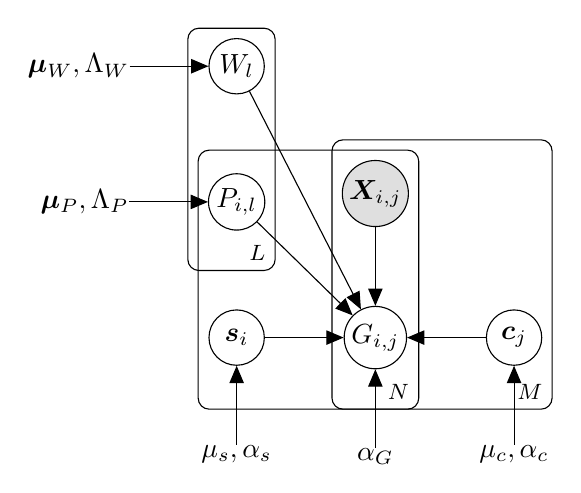
\begin{tikzpicture}

    % Define nodes
    \node[latent]                            (G) {$G_{i,j}$};
    \node[latent, left=of G]                 (s) {$\bm{s}_i$};
    \node[latent, right=of G]                (c) {$\bm{c}_j$};
    \node[latent, above=of s]                (P) {$P_{i,l}$};
    \node[latent, above=of P]                (W) {$W_l$};
    \node[obs, above=of G]                   (X) {$\bm{X}_{i,j}$};

    % G params
    \node[const, below=of G]  (pG) {$\alpha_G$};
    \edge {pG} {G};

    % s hyperparams
    \node[const, below=of s]  (Ts) {$\mu_s, \alpha_s$};
    \edge {Ts} {s};

    % c hyperparams
    \node[const, below=of c]  (Tc) {$\mu_c, \alpha_c$};
    \edge {Tc} {c};

    % P hyperparams
    \node[const, left=of P]   (TP) {$\bm{\mu}_P, \Lambda_P$};
    \edge {TP} {P};

    % W hyperparams
    \node[const, left=of W]   (TW) {$\bm{\mu}_W, \Lambda_W$};
    \edge {TW} {W};

    % Connect the nodes
    \edge {c,s,W,P,X} {G}; %

    % Plates
    \plate {student} {(s)(P)(G)(X)} {$N$};
    \plate {course} {(c)(G)(X)(student.north east)} {$M$};
    \plate {model} {(W)(P)(student.north west)} {$L$};

  \end{tikzpicture}
  \vspace{2pt}
  \caption{Bayesian PMLR Graphical Model} \label{fig:bpmlr-pgm}
\end{figure}


The likelihood of a particular grade $G_{i,j}$ is defined by:

\begin{equation}
    p(G | \bm{s}, \bm{c}, P, W, \alpha_G, \bm{X}) =
        \prod_{i=1}^n \prod_{j=1}^m
            \mathcal{N}(G_{i,j} | \hat{G}_{i,j}, \alpha_G),
\end{equation}

where

\begin{equation}
    \hat{G}_{i,j} = \bm{s}_i + \bm{c}_j + P_i^TW\bm{X}_{i,j}
\end{equation}

The four parameters $\bm{s}, \bm{c}, P, W$, and their hyperparameters are drawn
from the following distributions:

\begin{equation}
    p(\bm{s} | \mu_s, \alpha_s) =
        \prod_{i=1}^n \mathcal{N}(\bm{s}_i | \mu_s, \alpha_s)
\end{equation}

\begin{equation}
\begin{aligned}
    &p(\mu_s, \alpha_s | \mu_0, \kappa_0, \alpha_0, \beta_0) \\
        & = p(\mu_s | \alpha_s) p(\alpha_s) \\
        & = \mathcal{N}(\mu_s | \mu_0, (\kappa_0 \alpha_s))
            \Gamma(\alpha_s | \alpha_0, \beta_0)
\end{aligned}
\end{equation}

\begin{equation}
    p(\bm{c} | \mu_c, \alpha_c) =
        \prod_{j=1}^m \mathcal{N}(\bm{c}_j | \mu_c, \alpha_c)
\end{equation}

\begin{equation}
\begin{aligned}
    &p(\mu_c, \alpha_c | \mu_0, \kappa_0, \alpha_0, \beta_0) \\
        & = p(\mu_c | \alpha_c) p (\alpha_c) \\
        & = \mathcal{N}(\mu_c | \mu_0, (\kappa_0 \alpha_c))
            \Gamma(\alpha_c | \alpha_0, \beta_0)
\end{aligned}
\end{equation}

\begin{equation}
    p(P | \bm{\mu_P}, \Lambda_P) =
        \prod_{i=1}^n \mathcal{N}(P_i | \bm{\mu_P}, \Lambda_P)
\end{equation}

\begin{equation}
\begin{aligned}
    &p(\bm{\mu_P}, \Lambda_P | \bm{\mu_0}, \kappa_0, W_0, d_0) \\
        & = p(\bm{\mu_P} | \Lambda_P) p(\Lambda_P) \\
        & = \mathcal{N}(\bm{\mu_P} | \bm{\mu_0}, [\kappa_0 \Lambda_P])
            \mathcal{W}(\Lambda_P | W_0, d_0)
\end{aligned}
\end{equation}

\begin{equation}
    p(W | \bm{\mu_W}, \Lambda_W) =
        \prod_{l=1}^M \mathcal{N}(W_l | \bm{\mu_W}, \Lambda_W)
\end{equation}

\begin{equation}
\begin{aligned}
    &p(\bm{\mu_W}, \Lambda_W | \bm{\mu_0}, \kappa_0, W_0, d_0) \\
        & = p(\bm{\mu_W} | \Lambda_W) p(\Lambda_W) \\
        & = \mathcal{N}(\bm{\mu_W} | \bm{\mu_0}, [\kappa_0 \Lambda_W])
            \mathcal{W}(\Lambda_W | W_0, d_0)
\end{aligned}
\end{equation}


\subsection{Inference: Gibbs Sampler}

%% CPD for student bias vector: s
\begin{mdframed}[style=eqbox]
\begin{equation} \label{eqn:cpd-s}
\begin{aligned}
    &p(\bm{s}_i | \bm{c}, P, W, \bm{X}, G, \alpha_G, \Theta_s)
        = \mathcal{N}(\bm{s}_i | \mu_{s_i}^*, \alpha_{s_i}^*) \\
        & \sim \mathcal{N}(\bm{s}_i | \mu_s, \alpha_s)
               \prod_{j=1}^m \mathcal{N}(G_{i,j} | \hat{G}_{i,j}, \alpha_G)
\end{aligned}
\end{equation}

where

\begin{align}
    \alpha_{s_i}^* &= \begin{aligned}[t]
        \alpha_s + \alpha_G \sum_{j=1}^m I_{i,j}
    \end{aligned}\\
%
    \mu_{s_i}^* &= \begin{aligned}[t]
        \hstretch{0.8}{\vstretch{0.9}{
            \frac{\alpha_s\mu_s -
                  \alpha_G \sum_{j=1}^m
                      [\bm{c}_j + P_i^TW\bm{X}_{i,j} - G_{i,j} ] I_{i,j}}
                 {\alpha_{s_i}^*}}}
    \end{aligned}
\end{align}
\end{mdframed}
%% END: CPD for s


%% CPD for course bias vector: c
\begin{mdframed}[style=eqbox]
\begin{equation} \label{cpd-c}
\begin{aligned}
    &p(\bm{c}_j | \bm{s}, P, W, \bm{X}, G, \alpha_G, \Theta_c)
        = \mathcal{N}(\bm{c}_j | \mu_{c_j}^*, \alpha_{c_j}^*) \\
        & \sim \mathcal{N}(\bm{c}_j | \mu_c, \alpha_c)
               \prod_{i=1}^n \mathcal{N}(G_{i,j} | \hat{G}_{i,j}, \alpha_G)
\end{aligned}
\end{equation}

where

\begin{align}
    \alpha_{c_j}^* &= \begin{aligned}[t]
        \alpha_c + \alpha_G \sum_{i=1}^n I_{i,j}
    \end{aligned}\\
%
    \mu_{c_j}^* &= \begin{aligned}[t]
        \hstretch{0.8}{\vstretch{0.9}{
            \frac{\alpha_c\mu_c -
                  \alpha_G \sum_{i=1}^n
                      [\bm{s}_i + P_i^TW\bm{X}_{i,j} - G_{i,j} ] I_{i,j}}
                 {\alpha_{c_j}^*}}}
    \end{aligned}
\end{align}
\end{mdframed}
%% END: CPD for c


%% CPD for student membership matrix: P
\begin{mdframed}[style=eqbox]
{\setlength{\mathindent}{0cm}
\begin{equation} \label{cpd-P}
\begin{aligned}
    &p(P_i | \bm{s}, \bm{c}, W, \bm{X}, G, \Theta_P) =
        \mathcal{N}(P_i | \bm{\mu}_{P_i}^*, \Lambda_{P_i}^*) \\
        & \sim p(P_i | \bm{\mu_P}, \Lambda_P)
            \prod_{j=1}^m \mathcal{N}(G_{i,j} | \hat{G}_{i,j}, \alpha_G)
\end{aligned}
\end{equation}

where

\begin{align}
    \Lambda_{P_i}^* &= \begin{aligned}[t]
        \Lambda_P +
        \alpha_G W \left(
            \sum_{j=1}^m [\bm{X}_{i,j} \bm{X}_{i,j}^T ] I_{i,j}
        \right) W^T
    \end{aligned}\\
%
    \bm{\mu}_{P_i}^* &= \begin{aligned}[t]
        \vstretch{0.9}{\hstretch{0.8}{
            [\Lambda_{P_i}^*]^{-1} \left(
                \Lambda_P\bm{\mu_P} +
                \alpha_G W \sum_{j=1}^m
                    [\bm{X}_{i,j}(G_{i,j} - \bm{s}_i - \bm{c}_j)] I_{i,j}
            \right)}}
        \end{aligned}
\end{align}}
\end{mdframed}
%% END: CPD for P


%% CPD for regression coefficient matrix: W
\begin{mdframed}[style=eqbox]
{\setlength{\mathindent}{0cm}
\begin{equation} \label{cpd-W}
\begin{aligned}
    &p(W_l | \bm{s}, \bm{c}, P, \bm{X}, G, \Theta_W) =
        \mathcal{N}(W_l | \bm{\mu}_{W_l}^*, \Lambda_{W_l}^*) \\
        & \sim \mathcal{N}(W_l | \bm{\mu_W}, \Lambda_W)
            \sum_{i=1}^n \sum_{j=1}^m
                \mathcal{N}(G_{i,j} | \hat{G}_{i,j}, \alpha_G)
\end{aligned}
\end{equation}

where

\begin{align}
    \Lambda_{W_l}^* &= \begin{aligned}[t]
        \Lambda_W + \alpha_G \sum_{i=1}^N
            [ P_{i,l}^2 \sum_{j=1}^m
                \bm{X}_{i,j} \bm{X}_{i,j}^T ] I_{i,j}
    \end{aligned}\\
%
    \bm{\mu}_{W_l}^* &= \begin{aligned}[t]
        \vstretch{0.8}{\hstretch{0.7}{
            [\Lambda_{W_l}^*]^{-1} \left(
                \Lambda_W\bm{\mu_W} +
                \alpha_G \sum_{i=1}^n
                    [P_{i,l} \sum_{j=1}^m
                        \bm{X}_{i,j}(G_{i,j} - \bm{s}_i - \bm{c}_j)
                    ] I_{i,j}
            \right)}}
    \end{aligned}
\end{align}}
\end{mdframed}
%% END: CPD for W


\section{Derivations}\label{derivations}

\setlength{\belowdisplayskip}{6pt} \setlength{\belowdisplayshortskip}{6pt}
\setlength{\abovedisplayskip}{8pt} \setlength{\abovedisplayshortskip}{8pt}

In this section, derivations for the semi-conjugate posterior distributions of P
and W are given. First we show derivations for a simplified version of the model
without the bias terms, so we have:
%
\begin{equation}
    \hat{G}_{ij} = P_i^T W X_{ij}
\end{equation}
%
\begin{flalign}
    &p(P | W, \bm{X}, \mu_P, \Lambda_P)  \\
        \nonumber
        &= \prod_{i=1}^N \mathcal{N}(P_i | \mu_P, \Lambda_P)
           \prod_{j=1}^M \mathcal{N}(G_{ij} | \hat{G}_{ij}, \alpha_G) \\
%
    &p(W | P, \bm{X}, \mu_W, \Lambda_W)  \\
        \nonumber
        &=  \prod_{l=1}^L\mathcal{N}(W_l | \mu_W, \Lambda_W)
            \prod_{i=1}^N \prod_{j=1}^M
                \mathcal{N}(G_{ij} | \hat{G}_{ij}, \alpha_G)
\end{flalign}
%
So for a single row $P_i$, we have conditional distribution:
%
\begin{flalign}
    &p(P_i | W, \bm{X}, \mu_P, \Lambda_P)  \\
    \nonumber
    &=  \mathcal{N}(P_i | \mu_P, \Lambda_P)
        \prod_{j=1}^M \mathcal{N}(G_{ij} | \hat{G}_{ij}, \alpha_G) \\
%%
    \nonumber
    &= \frac{|\Lambda_P|^{1/2}}{(2\pi)^{f/2}}
        exp\left\{
            -\frac{1}{2} (P_i - \mu_P)^T \Lambda_P (P_i - \mu_P)
        \right\} \\
        &\hspace{4mm}\vspace{-2mm} \times
        \frac{|\alpha_G|^{M/2}}{(2\pi)^{Mf/2}}
        exp\left\{
            -\frac{\alpha_G}{2} \sum_{j=1}^M (G_{ij} - \hat{G}_{ij})^2
        \right\} \\
%%
    &\propto
        (P_i - \mu_P)^T \Lambda_P (P_i - \mu_P) +
        \alpha_G \sum_{j=1}^M (G_{ij} - \hat{G}_{ij})^2 \\
%%
    &=  (P_i^T\Lambda_P - \mu_P^T\Lambda_P) (P_i - \mu_P) +
        \alpha_G \sum_{j=1}^M (G_{ij} - \hat{G}_{ij})^2 \\
%%
    \nonumber
    &=  P_i^T \Lambda_P P_i - 2 P_i^T \Lambda_P \mu_P + \mu_P^T \Lambda_P \mu_P \\
        &\hspace{4mm}\vspace{-2mm}
        + \alpha_G \sum_{j=1}^M
            (G_{ij}^2 - 2 G_{ij} \hat{G}_{ij} + \hat{G}_{ij}^2) \\
%%
    \nonumber
    &\propto
        P_i^T \Lambda_P P_i - 2 P_i^T \Lambda_P \mu_P \\
        &\hspace{4mm}\vspace{-2mm}
        + \alpha_G \sum_{j=1}^M \left(
            (P_i^T W X_{ij})^2 - 2 G_{ij} (P_i^T W X_{ij})
        \right) \\
%%
    \nonumber
    &=  P_i^T \left(
        \Lambda_P + \alpha_G \sum_{j=1}^M (W X_{ij})(W X_{ij})^T
        \right) P_i \\
        &\hspace{4mm}\vspace{-2mm}
        - 2 P_i^T \left(
            \Lambda_P \mu_P + \alpha_G \sum_{j=1}^M G_{ij} W X_{ij}
        \right) \\
%%
    \nonumber
    &=  P_i^T \left(
            \Lambda_P + \alpha_G W \left(
                \sum_{j=1}^M X_{ij} X_{ij}^T
            \right) W^T
        \right) P_i \\
        &\hspace{4mm}\vspace{-2mm}
        - 2 P_i^T \left(
            \Lambda_P \mu_P + \alpha_G W \sum_{j=1}^M G_{ij} X_{ij}
        \right) \\
%%
    &\propto
        \mathcal{N}(P_i | \mu_{P_i}^*, \Lambda_{P_i}^*),
\end{flalign}
%
where
%
\begin{align}
    \Lambda_{P_i}^* &= \begin{aligned}[t]
        \Lambda_P + \alpha_G W \left[\sum_{j=1}^M
            [X_{ij} X_{ij}^T] I_{ij}
        \right] W^T
    \end{aligned}\\
%
    \bm{\mu}_{P_i}^* &= \begin{aligned}[t]
        \vstretch{0.9}{\hstretch{0.8}{
            [\Lambda_{P_i}^*]^{-1} \left[
                \Lambda_P\bm{\mu_P} +
                \alpha_G W \sum_{j=1}^M [G_{ij} X_{ij}] I_{ij}
            \right]}}
    \end{aligned}
\end{align}
%% END: CPD for P

Next we look at the conditional distribution for $W$ given everything else.
Recall that we are working with the version of the model without bias terms.
Using the result for $P$, we can skip a few steps. For each model $l = \{1, ...,
L\}$, we have:
%
\begin{align}
    &p(W_l | \mu_W, \Lambda_W) \\
    \nonumber
    &\propto
        exp\left\{
            -\frac{1}{2} (W_l - \mu_W)^T \Lambda_W (W_l - \mu_W)
        \right\} \\
        &\hspace{4mm}\vspace{-2mm} \times
        exp\left\{
            -\frac{\alpha_G}{2} \sum_{i=1}^N \sum_{j=1}^M
                (G_{ij} - \hat{G}_{ij})^2
        \right\} \\
%%
    \nonumber
    &\propto
        W_l^T \Lambda_W W_l - 2 W_l^T \Lambda_W \mu_W \\
        &\hspace{4mm}\vspace{-2mm}
        + \alpha_G \sum_{i=1}^N \sum_{j=1}^M
        ((P_i^T W X_{ij})^2 - 2 G_{ij} (P_i^T W X_{ij})) \\
%%
    \nonumber
    &=  W_l^T \Lambda_W W_l - 2 W_l^T \Lambda_W \mu_W \\
        &\hspace{4mm}\vspace{-2mm}\nonumber
        + \alpha_G \sum_{i=1}^N \sum_{j=1}^M \left(
            \sum_{l'=1}^L (P_{il'} W_{l'} X_{ij})^2 \right. \\
            &\hspace{28mm}\vspace{-2mm}\left.
            - 2 G_{ij} X_{ij} \sum_{l'=1}^L (P_{il'} W_{l'})
        \right) \\
%%
    \nonumber
    &\propto
        W_l^T \Lambda_W W_l - 2 W_l^T \Lambda_W \mu_W \\
        &\hspace{4mm}\vspace{-2mm}\nonumber
        + \alpha_G \sum_{i=1}^N \sum_{j=1}^M (P_{il} W_l X_{ij})^2 \\
        &\hspace{4mm}\vspace{-2mm}
        - 2 \alpha_G \sum_{i=1}^N \sum_{j=1}^M G_{ij} P_{il} W_l X_{ij} \\
%%
    \nonumber
    &=  W_l^T \left(
            \Lambda_W + \alpha_G \sum_{i=1}^N P_{il}^2
                        \sum_{j=1}^M X_{ij} X_{ij}^T
        \right) W  \\
        &\hspace{4mm}\vspace{-2mm}
        - 2 W_l^T \left(
            \Lambda_W \mu_W + \alpha_G \sum_{i=1}^N P_{il}
                              \sum_{j=1}^M G_{ij} X_{ij}
        \right) \\
%%
    &\propto
        \mathcal{N}(W_l | \bm{\mu}_{W_l}^*, \Lambda_{W_l}^*),
\end{align}
%
where
%
\begin{align}
    \Lambda_{W_l}^* &= \begin{aligned}[t]
        \Lambda_W + \alpha_G \sum_{i=1}^N P_{il}^2 \sum_{j=1}^M
            [X_{ij} X_{ij}^T] I_{ij}
    \end{aligned}\\
%
    \bm{\mu}_{W_l}^* &= \begin{aligned}[t]
        \vstretch{0.9}{\hstretch{0.8}{
            [\Lambda_{W_l}^*]^{-1} \left[
                \Lambda_W\bm{\mu}_W +
                \alpha_G \sum_{i=1}^N P_{il} \sum_{j=1}^M
                    [G_{ij} X_{ij}] I_{ij}
            \right]}}
    \end{aligned}
\end{align}
%% END: CPD for W


\section{Previous work}\label{previous work}


\section{Results}\label{results}
In this section we describe the results.


\section{Conclusions}\label{conclusions}
We worked hard, and achieved very little.


% use section* for acknowledgement
\section*{Acknowledgment}
This research was funded by NSF IIS grant 1447489.


\bibliographystyle{siam}
\bibliography{refs}

\end{document}

